\documentclass[a4paper,10pt]{report}
\usepackage[frenchb]{babel}
\usepackage[utf8]{inputenc}
\usepackage[T1]{fontenc}
\usepackage{graphicx}
\usepackage{mathenv}
\usepackage{algpseudocode}
\usepackage{float}
\usepackage{hyperref}
\usepackage[final]{pdfpages} 
\usepackage{changepage}
\usepackage{graphicx}

\usepackage{array}

\usepackage{caption}

\usepackage[linesnumbered,ruled]{algorithm2e}

\usepackage{amssymb}

\newcounter{cnt}
\newcommand{\definition}{
  \addtocounter{cnt}{1}
 \textbf{Définition}
}



% Title Page
\title{Université d'Angers \\  \emph{M2 Intelligence Décisionnelle \\} \hrulefill \\ \textbf{Recherche de motifs fréquents par algorithmes évolutionnaires} \\ \hrulefill}
\author{Ugo Rayer}


\begin{document}

    \begin{titlepage}

\newcommand{\HRule}{\rule{\linewidth}{0.5mm}}

\center 

\textsc{\LARGE Université d'Angers}\\[1.5cm] 
\textsc{\Large M2 Intelligence Décisionnelle}\\ [0.5cm] 
\textsc{\large }\\[0.5cm] 


\HRule \\[0.4cm]
{ \huge \bfseries Recherche de motifs fréquents par algorithmes évolutionnaires}\\[0.4cm] 
\HRule \\[1.5cm]
 

\begin{minipage}{0.4\textwidth}
\begin{flushleft} \large
\emph{Auteur:}\\
Ugo \textsc{Rayer} 
\end{flushleft}
\end{minipage}
~
\begin{minipage}{0.4\textwidth}
\begin{flushright} \large
\hfill
\begin{tabular}{@{}l@{}}
\emph{Encadrants:}\\
Benoit \textsc{Da Mota} \\
Béatrice \textsc{Duval} \\
David \textsc{Lesaint} 
\end{tabular}
\end{flushright}
\end{minipage}\\[4cm]



{\large \today}\\[3cm] 




\includegraphics{./img/ua.jpg}\\[1cm]

\vfill 

\end{titlepage}

\newpage
~
\newpage
\chapter*{Remerciements}

Avant toute chose, je tiens à remercier l'ensemble des personnes qui ont participé, de près ou de loin, à la réalisation de ce stage et à l'écriture de ce rapport. \\

\hspace{0.2cm}Des remerciements spéciaux sont adressés d'une part au Laboratoire d'Etude et de Recherche en Informatique d'Angers pour son accueil et d'autre part au projet GRIOTE de la région Pays de la Loire qui a financé cette étude. Ensuite, je tiens à remercier chaleureusement Madame Duval et Messieurs Da Mota et Lesaint pour la qualité de leur encadrement et les différentes remarques qu'ils m'ont prodiguées pendant ces quelques mois. \\

\hspace{0.2cm}Enfin, un grand merci à Josépha pour ses précieux conseils d'écriture malgré l'incompréhension générale des sujets abordés.

\tableofcontents
\newpage

\chapter{Introduction}
Le calcul des motifs fréquents est une notion essentielle dans de nombreux domaines liés à la découverte et l'extraction de connaissances. Initiallement introduit par Agrawal et al. dans \cite{AGR93}, ces motifs étaient alors utilisés pour l'établissement de règles d'associations visant à caractériser les habitudes d'achats de clients d'un supermarché. Par exemple, une règle de la forme "Pain \& Beurre $\Rightarrow$ Jambon (75\%)" signifie que 3 clients sur 4 achetant du pain et du beurre achètent également du jambon. Le calcul de telles règles se fait en deux étapes, dont la principale (i.e. disposant de la plus grosse complexité calculatoire) correspond au calcul des motifs fréquents. Depuis son introduction, le problème du calcul des motifs fréquents a été très largement étudié et appliqué à de nombreux domaines comme en bio-informatique, en cybersécurité et bien évidemment en marketing.\\

\hspace{0.15cm}L'avènement de l'ère du Big Data a fait rentrer le problème de calcul des motifs fréquents dans une nouvelle dimension. En effet, le volume de données produites dans tous les domaines a cru de manière vertigineuse ces dernières années, rendant l'extraction de connaissances d'autant plus nécessaire et délicate. De fait, la problématique du passage à l'échelle des méthodes exactes est devenue primordiale. Bien que divers efforts en ce sens aient été faits au travers de nombreuses publications, ils se concentrent généralement sur l'optimisation et la parallélisation des méthodes existantes. \\

\hspace{0.15cm}Les algorithmes évolutionnaires font partie des techniques de résolution de problèmes combinatoires appelées méta-heuristiques. Les méta-heuristiques regroupent un ensemble de méthodes approchées à la résolution de problème combinatoire. Elles sont naturellement envisagée lorsque la complexité du problème étudié ne permet pas l'usage de méthodes exactes (aussi bien en temps qu'en espace). Le principe des algorithmes évolutionnaires est de manipuler un ensemble d'individus représentant chacun une solution au problème étudié. A chaque itération, certains individus sont modifiés via des opérateurs de croisement et de mutation. Chaque individu est évalué au regard d'une fonction à optimiser dépendant du problème étudié. \\

\hspace{0.15cm}Ainsi, nous formaliserons le problème de calcul de motifs fréquents dans la section suivante avant d'effectuer un état de l'art des méthodes existantes en section 3. Le chapitre 4 sera dédié à la présentation de notre méthode dont nous présenterons les résultats en section 5. Le dernier chapitre sera consacré à la conclusion de cette étude et à une ouverture vers de futurs travaux.

\newpage
\chapter{Le problème du calcul motifs fréquents}

\section{Définition du problème}
	La définition la plus courante du problème de calcul des motifs fréquents se fait par la théorie des ensembles. Nous verrons cependant dans le chapitre suivant qu'il peut également être décrit par la théorie des graphes. Nous présenterons dans un premier temps un cadre formel nécessaire à la définition du problème que nous illustrerons ensuite. Enfin, nous introduirons quelques propriétés dérivés de la définition du problème.

\subsection{Formalisation}
	Soit $\mathcal{I}$ un ensemble de \emph{symboles} appelées \textbf{items}. Quelque soit \emph{I} $ \subseteq \mathcal{I}$, \emph{I} est un \emph{motif} appelé \textbf{itemset}. \\

\hspace{0.15cm}Soit $\mathcal{T}$ = \{ \emph{$t_{1}$, ... , $t_{n}$ } \} un ensemble de \textbf{transactions}. Chaque élément \emph{$t_{i}$} est un couple $< tid, \emph{I} >$ où \emph{tid} est l'identifiant de la transaction et \emph{I} $\subseteq \mathcal{I}$. $\mathcal{T}$ est communément appelé \textbf{base de transactions}.  \\

\hspace{0.15cm}Pour tout itemset \emph{I} $\subseteq \mathcal{I}$ la \textbf{couverture} de \emph{I} par $\mathcal{T}$ est définie par : \\
\begin{center}
\textbf{cover$_{\mathcal{T}}$}(\emph{I}) = \{ \emph{t} $\in \mathcal{T}  | \emph{ I} \subseteq \emph{t }\}$
\end{center}

\hspace{0.15cm}La cardinalité de la couverture d'un itemset \emph{I} par $\mathcal{T}$ \\
\begin{center}
\textbf{sup$_{\mathcal{T}}$}(\emph{I}) = $|$ \textbf{cover$_{\mathcal{T}}$}(\emph{I}) $|$
\end{center}
est appelée \textbf{support} de \emph{I}.  Etant donné un support minimal \emph{minsup} l'ensemble des \textbf{itemsets} (i.e. motifs) \textbf{fréquents} est défini par : \\
\begin{center}
$\textbf{F}_{\mathcal{T},minsup}$ = \{ \emph{I} $\subseteq \mathcal{I } |$  $sup_{\mathcal{T}}(\emph{I}) \geq$ \emph{minsup} \}
\end{center}

\hspace{0.15cm}Le problème du \textbf{calcul des itemsets fréquents} ( \textbf{FIM} - \emph{Frequent Itemsets Mining}) est, étant donné une base de transactions $\mathcal{T}$ et un support minimal \emph{minsup} de calculer l'ensemble \emph{F} des itemsets fréquents. Comme F. Boden le remarque dans \cite{BOD06}, bien qu'historiquement définie comme une valeur relative et donc asujettie à un support minimal défini dans l'intervalle [0,1], le support est de nos jours mesuré de manière absolue. Si nécessaire, nous y ferons référence sous la notion de fréquence : \\
\begin{center}
$\textbf{Freq}_{\mathcal{T}}$(\emph{I}) = $\frac{ | \textbf{ cover$_{\mathcal{T}}$}(\emph{I})  | } { | \mathcal{T} | }$
\end{center}
avec \emph{minfreq} simplement définie par $\frac{\emph{minsup}}{| \mathcal{T} |}$. \\

\subsection{Exemple}
	Situons nous dans le contexte de la définition historique de problème et considérons la base de transactions suivante (que nous conserverons tout au long de cet article). Le tableau 1 décrit chaque transaction par : un identifiant, une liste d'objets achetés et la liste des items fréquents vis à vis d'un support minimal de  3.\\

\begin{tabular}{|c|l|l|}
	\hline
	ID transaction & Objets achetés & Items Fréquents Ordonnés \\
	\hline
	100 & f, c, a, d, g, i m, p & f, c, a, m, p \\
	\hline
	200 & a, b, c, f, l, m, o & f, c, a, b, m \\
	\hline
	300 & b, f, h, j, o & f, b \\
	\hline
	400 & b, c, k, s, p & c, b, p \\
	\hline
	500 & a, f, c, e, l, p, m, n & f, c, a, m, p \\
	\hline	
\end{tabular}
\captionof{table}{Base de transactions exemple}
\vspace{0.4cm}

\hspace{0.15cm}Une fois calculé, l'ensemble des itemsets fréquents vis à vis de ce jeu de données $\mathcal{T}$ est l'ensemble $\textbf{F}_{\mathcal{T},3}$ = \{ (f:4), (c:4), (a:3), (b:3), (m:3), (p:3), (fc:3), (fa:3), (fm:3), (cm:3), (cp:3), (ca:3), (am:3), (fca:3), (fcm:3), (fam:3), (cam:3), (fcam:3) \}.  \\

\subsection{Complexité et Propriétés}
La complexité du problème vient d'une part du nombre d'itemsets à considérer en fonction du nombre d'objets et d'autre part de nombre de transactions dans la base. En effet, soit \emph{n} objets fréquents dans la base, il y a alors $2^{n}$ itemsets possibles. D'autre part, le calcul du support d'un itemset se fait au travers de l'ensemble des transactions. L'efficacité d'une méthode à résoudre ce problème se fera donc par sa capacité à explorer intelligement l'espace des $2^{n}$ itemsets et par son efficacité à calculer le support d'un itemset vis à vis de $| \mathcal{T} |$. \\
\hspace{0.15cm}Différents théorèmes et propriétés issus de l'étude de ce problème sont utilisés dans les méthodes proposées pour le résoudre. Nous présentons les propriétés liées à la monotonie du support d'un ensemble et renvoyons le lecteur vers \cite{BOD06} et \cite{GOE} pour plus de détails. \\
\textbf{Monotonie du support.} Soit une base de transactions $ \mathcal{T} sur \mathcal{I} $ et soient \emph{X, Y} $\subseteq \mathcal{I}$ deux itemsets. Alors, \\
\begin{center}
\emph{X} $\subseteq $ \emph{Y} $\Rightarrow$ \textbf{sup$_{\mathcal{T}}$}(\emph{Y}) $ \leq $ \textbf{sup$_{\mathcal{T}}$}(\emph{X})
\end{center}

Cette propriété nous permet de dire que si un k-itemset \emph{X} (i.e. un itemset comprenant k objets) est fréquent, alors l'ensemble \emph{Y} des k-1-itemsets $\subset $\emph{X} est fréquent. Par exemple, (fca:3) est fréquent, de même que (fc:3), (fa:3) et (ca:3). Nous pouvons de manière duale dire que si un k- itemset \emph{X} est non-fréquent, alors aucun des k+1-itemset \emph{Y} tel que \emph{X} $ \subset $ \emph{Y} n'est fréquent. Ces deux observations sont à la base des différents sens de parcours de l'espace de recherche des $2^{n}$ itemsets possibles dans la plupart des algorithmes.

\section{Problème des itemsets clos maximaux}

	Afin de réduire l'espace de recherche, il a été proposé de contraindre la recherche à l'ensemble des itemsets clos. Un k-itemset\emph{X} fréquent est clos si \textbf{sup$_{\mathcal{T}}$}(\emph{X}) $>$ \textbf{sup$_{\mathcal{T}}$}(\emph{Y}) $ \forall  $ \emph{Y} tel que \emph{X} $ \subset $ \emph{Y}.  Un itemset clos est maximal si aucun de ses surensembles n'est fréquent. Ainsi dans notre exemple, l'ensemble des itemsets clos est   $\textbf{C}_{\mathcal{T},3}$ = \{ (f:4), (c:4), (b:3), (cp:3), (fcam:3) \} et l'ensemble des itemsets clos maximaux est  $\textbf{MC}_{\mathcal{T},3}$ =  $\textbf{C}_{\mathcal{T},3} - $ \{ (f:4), (c:4) \}. La figure suivante représente le treillis complet des différents itemsets possibles sur les objets fréquents. Y figurent d'une part les itemsets fréquents en vert, d'autre part les itemsets clos en jaune et enfin les itemsets clos maximaux en rouge. Pour plus de lisibilité, les itemsets non-fréquents ne figurent pas dans le treillis.\\

\begin{figure}
	\begin{adjustwidth}{-2.7cm}{}
	\begin{tabular}{l}
	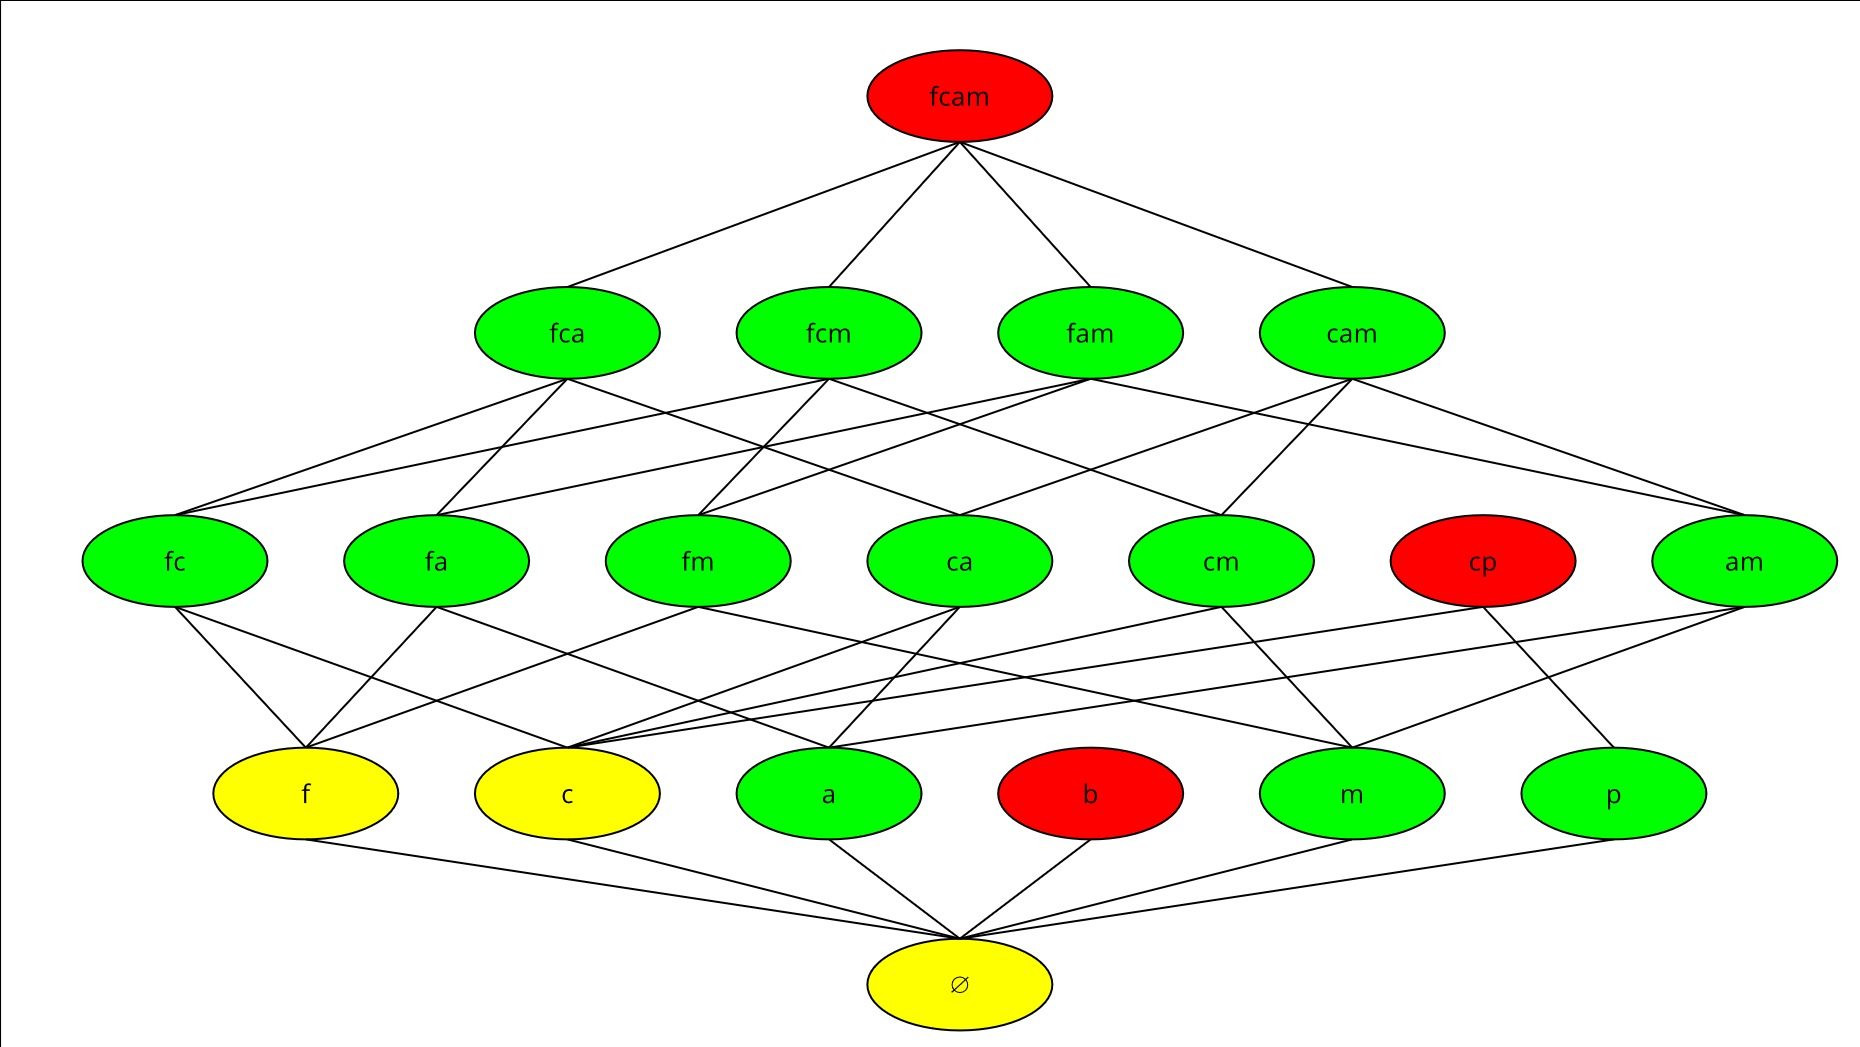
\includegraphics[width=12cm,height=10cm]{./img/treillis_is.jpg}\\
	\end{tabular}
	\caption{\label{fig:text}Treillis des itemsets fréquents, clos et maximaux de notre exemple}
	\end{adjustwidth}
\end{figure}

Zaki et al. et Pas. et al. prouvent dans \cite{ZAK99} et \cite{PAS99} que l'intégralité des itemsets fréquents peut être dérivée de l'ensemble des itemsets clos maximaux. Ils proposent alors d'adapter les méthodes existantes pour le calcul des itemsets clos maximaux. 

\newpage

\section{Itemset et classification}

	Dans cette section nous redéfinissons le problème à considérer. Nous l'étudierons ensuite sous l'aspect d'un problème combinatoire solvable par recherche locale. Enfin nous l'aborderons via une approche évolutionnaire. \\

\subsection{Définition du problème}
	Soit $\mathcal{T}$ une base de transactions définie sur $\mathcal{N}$ items. En plus d'un identifiant et de ses items, chaque transaction possède une classe (positive ou négative). Le problème consiste à trouver parmi $\mathcal{T}$ un itemset X tel que le support de X dans la classe positive soit supérieur à un seuil minimal \emph{minsup} \textbf{et} que le support de X dans la classe négative soit inférieur à un seuil maximal \emph{maxsup}. \\

	Formellement, soit X = \{$i_{1}, ..., i_{k}$\} un k-itemset quelconque. Alors, soient \textbf{$sup_{+}$}(X) et \textbf{$sup_{-}$}(X) les deux fonctions suivantes : 
\begin{center}
\textbf{$sup_{+}$}(X) = \{$t_{j}$ | $t_{j} \in \mathcal{T}$ et $\forall i \in X,  t_{i,j}$ = 1 et $t_{j} \in C^{+}$\}\\ 
\textbf{$sup_{-}$}(X) = \{$t_{j}$ | $t_{j} \in \mathcal{T}$ et $\forall i \in X,  t_{i,j}$ = 1 et $t_{j} \in C^{-}$\}\\ 
\end{center}
X est un itemset solution si et seulement si les propriétés suivantes sont vérifiées : 
\begin{center}
|\textbf{$sup_{+}$}(X)| > \emph{minsup}\\
|\textbf{$sup_{-}$}(X)| < \emph{maxsup}\\
\end{center}

Nous sommes donc confronté à un problème de classification visant à trouver l'itemset permettant la meilleure discrimination entre les classes positives et négatives. 

\subsection{Représentation et évaluation d'une solution}

	Le problème étant de trouver un itemset maximisant la couverture de la classe positive tout en minimisant son support dans la classe négative, une solution du problème est simplement un bitset \emph{S} de $\mathcal{N}$ bits tel que $\forall \emph{i} \in [1..\mathcal{N}] \emph{S}_{i} = 1$ si l'item \emph{i} appartient à la solution, $\emph{S}_{i}$ = 0 sinon. \\
	L'évaluation d'une solution doit permettre de quantifier la corrélation des différents items dans leur pouvoir de classification de la base de transactions. Diverses mesures existent et ont été proposées et largement étudiées dans la littérature (citation TAN02, GEN06, ...).\\
	Nous proposons dans un premier temps d'utiliser la \emph{F-Mesure}, correspondant à la moyenne harmonique entre précision et rappel. Ces deux mesures sont calculées à partir des résultats de la classification de $\mathcal{T}$ par une solution \emph{S}. Chaque transaction \emph{t} appartient à un des quatre ensembles suivants : 
\begin{center}
	- Vrai positif (TP) : $\forall \emph{i} \in [1..\mathcal{N}]$  $\emph{S}_{i} = 1 et \emph{t}_{i} = 1$ \&  $\emph{t} \in C^{+}$ \\
	- Faux Positif (FP) : $\exists \emph{i} \in [1..\mathcal{N}]$ tel que $\emph{S}_{i} = 1, \emph{t}_{i} = 0$ \&  $\emph{t} \in C^{+}$\\
	- Vrai Négatif (TN) : $\exists \emph{i} \in [1..\mathcal{N}]$ tel que $\emph{S}_{i} = 1, \emph{t}_{i} = 0$ \&  $\emph{t} \in C^{-}$\\
	- Faux Négatif (FN) : $\forall \emph{i} \in [1..\mathcal{N}]$ $\emph{S}_{i} = 1, \emph{t}_{i} = 1$ \&  $\emph{t} \in C^{-}$\\
\end{center}

 Le tableau suivant récapitule l'appartenance d'une transaction \emph{t} à un des quatre ensembles : 
	 
\begin{center}
	\begin{tabular}{|c|c|c|}
		\hline
		& $\emph{S} \subseteq \emph{t}$ & $\emph{S} \not\subseteq \emph{t}$ \\
		\hline
		Classe \emph{t} = 1 & $\emph{t} \in TP$ & $\emph{t} \in FP$ \\
		\hline
		Classe \emph{t} = 0 & $\emph{t} \in FN$ & $\emph{t} \in TN$ \\
		\hline
\end{tabular}
\end{center}

La précision d'une telle classification correspond au rapport entre le nombre de réponses pertinentes données (TP) et le nombre de réponses données (TP+FP). Le rappel correspond quant à lui au rapport entre le nombre de réponses pertinentes données (TP) et le nombre de réponses pertinantes existant (TP+FN). 

\begin{center}
- Precision = $\frac{TP}{TP+FP}$ \\
\vspace{0.15cm}
- Rappel = $\frac{TP}{TP+FN}$\\
\end{center}

La \emph{F Mesure} permet d'aggréger rappel et précision en accordant un poids équivalent à chaque mesure. Cette une version simplifié de la \emph{$F_{\beta}$ Mesure} définie par la relation suivante : 
\begin{center}
- \emph{$F_{\beta}$} = (1+$\beta^{2}$) * $\frac{Precision*Rappel}{\beta^{2}*Precision + Rappel}$
\end{center}

Dans notre cas, où rappel et précision sont équitablement pondérés, la mesure peut se simplifier comme suit :
La \emph{F Mesure} permet d'aggréger rappel et précision en accordant un poids équivalent à chaque mesure. Cette une version simplifié de la \emph{$F_{\beta}$ Mesure} définie par la relation suivante : 
\begin{center}
- \emph{$F_{1}$} = $\frac{2*TP}{2*TP + FN + FP }$
\end{center}

\end{document}